% !TEX program = lualatex
% =====================================================================
%  离散数学期末课程报告
%  主题：图的色多项式及其递推计算
%  编译：lualatex report.tex （需 ctex 与 common/macros.tex）
% =====================================================================
\documentclass[10pt]{article}

% --- 页面：尽量利用纸面（沿用本项目紧凑设置） ----------------------
\usepackage{geometry}
\geometry{margin=1.5cm, vmargin={0pt,1cm}}
\setlength{\topmargin}{-1cm}
\setlength{\headheight}{14pt}
\setlength{\paperheight}{29.7cm}
\setlength{\textheight}{25.3cm}

% --- 中文、字体、页眉、绘图 ----------------------------------------
\usepackage[UTF8]{ctex}
\usepackage{fancyhdr}
\usepackage{tikz}
\usetikzlibrary{arrows.meta,positioning,calc,fit,shapes.geometric}
\usepackage{booktabs}

% --- 公共宏（定理环境、数学符号、中文支持等） ----------------------
% % % % % % % % % % % % % % % % % % % % % % % % % % % % % % % %
% Common Macros for LaTeX
% % % % % % % % % % % % % % % % % % % % % % % % % % % % % % % %

% Useful packages
\usepackage{amsfonts}
\usepackage{amsmath}
\usepackage{amssymb}
\usepackage{amsthm}
\usepackage{enumerate}
\usepackage{graphicx}
\usepackage{multicol}
\usepackage[ruled,linesnumbered]{algorithm2e}

% Math operators and common symbols
\newcommand{\dif}{\mathrm{d}}
\newcommand{\innerProd}[1]{\left\langle #1 \right\rangle}
\newcommand{\difFrac}[2]{\frac{\dif #1}{\dif #2}}
\newcommand{\pdfFrac}[2]{\frac{\partial #1}{\partial #2}}
\newcommand{\T}{\mathrm{T}}
\newcommand{\norm}[1]{\left\| #1 \right\|}
\newcommand{\abs}[1]{\left| #1 \right|}

% Vector and Matrix shortcuts
\newcommand{\vecTwo}[2]{
  \begin{bmatrix}
    #1 \\
    #2
\end{bmatrix}}
\newcommand{\vecThree}[3]{
  \begin{bmatrix}
    #1 \\
    #2 \\
    #3
\end{bmatrix}}
\newcommand{\vecTwoH}[2]{
  \begin{bmatrix}
    #1 & #2
  \end{bmatrix}
}
\newcommand{\vecThreeH}[3]{
  \begin{bmatrix}
    #1 & #2 & #3
  \end{bmatrix}
}

% Common fields
\newcommand{\R}{\mathbb{R}}
\newcommand{\C}{\mathbb{C}}
\newcommand{\Z}{\mathbb{Z}}
\newcommand{\N}{\mathbb{N}}

% Solutions and proofs
\newenvironment{solution}{
\begin{proof}[解]}{
\end{proof}}

% Utility to get environment variables (requires lualatex)
\newcommand{\getEnv}[2]{\directlua{tex.print(os.getenv("#1") or "#2")}}


% --- 紧凑排版参数（压至 3 页） -------------------------------------
\linespread{0.92}
\setlength{\parskip}{2pt plus 1pt minus 0.5pt}
\setlength{\abovedisplayskip}{4pt plus 2pt minus 1pt}
\setlength{\belowdisplayskip}{4pt plus 2pt minus 1pt}
\setlength{\abovedisplayshortskip}{2pt plus 1pt}
\setlength{\belowdisplayshortskip}{2pt plus 1pt}
\setlength{\textfloatsep}{6pt plus 2pt minus 2pt}
\setlength{\intextsep}{6pt plus 2pt minus 2pt}
\setlength{\floatsep}{6pt plus 2pt minus 2pt}
\makeatletter
\renewcommand\@listi{\leftmargin\leftmargini
  \topsep 3\p@\@plus1\p@\@minus1\p@
  \parsep \z@\@plus\p@
  \itemsep 1\p@\@plus\p@}
\let\@listI\@listi
\renewcommand\section{\@startsection{section}{1}{\z@}%
  {-2.6ex\@plus -0.8ex\@minus -0.2ex}{1.1ex\@plus.2ex}%
  {\normalfont\large\bfseries}}
\renewcommand\subsection{\@startsection{subsection}{2}{\z@}%
  {-2ex\@plus -0.6ex\@minus -0.2ex}{0.7ex\@plus.2ex}%
  {\normalfont\normalsize\bfseries}}
\makeatother

% --- 本报告专用宏 ---------------------------------------------------
\newcommand{\chrom}[2]{P_{#1}(#2)}        % 色多项式 \chrom{G}{k}
\newcommand{\chrnum}{\chi}                % 色数 \chi(G)

% --- tikz 图形样式 --------------------------------------------------
\tikzset{
  gv/.style={circle,draw,fill=white,inner sep=1pt,minimum size=3.8mm,
             font=\scriptsize},
  every picture/.style={line cap=round,line join=round}}

% --- 姓名 / 学号（用环境变量 NAME / UID 替换） ----------------------
\newcommand{\name}{\getEnv{NAME}{NAME}}
\newcommand{\uid}{\getEnv{UID}{UID}}

\begin{document}
\pagestyle{fancy}
\fancyhead{}
\lhead{\name\ (\uid)}
\chead{离散数学期末课程报告}
\rhead{\today}

% =====================================================================
\begin{center}
  {\Large\bfseries 图的色多项式及其递推计算}\\[2pt]
  {\footnotesize \name\quad\uid \quad\textbar\quad 离散数学}
\end{center}

\noindent\hrulefill
\begin{quote}\small
\textbf{摘要.}\, 图着色通常只问“能否用 $k$ 种颜色正常染色”。如果把问题换成“有多少种合法方案”，
就得到一个计数问题，而它的答案恰好是关于颜色数 $k$ 的多项式 $P_G(k)$，称为图的色多项式。
本文给出色多项式的定义和基本性质，围绕删除—收缩递推 $P_G(k)=P_{G-e}(k)-P_{G/e}(k)$ 展开，
算出完全图、树、环图等几类常见图的色多项式并给出具体算例，再看它的系数与图本身的结构有什么关系。
\end{quote}
\noindent\hrulefill

% =====================================================================
\section{引言：从图着色到计数}
% =====================================================================

设 $G=(V,E)$ 为简单无向图。其\textbf{正常 $k$-着色}是映射 $f:V\to\{1,\dots,k\}$，
满足 $\forall uv\in E,\ f(u)\ne f(v)$；\textbf{色数} $\chrnum(G)$ 是存在正常着色的最小颜色数。
传统着色问题只关心判定：“$\chrnum(G)\le k$ 是否成立？”本文要问的是它的计数版本：
给定 $k$ 种颜色，图 $G$ 一共有多少种正常着色？把这个数目记作 $P_G(k)$，可以证明它一定是 $k$
的多项式，称为色多项式（Birkhoff, 1912）。这样一来，原来的判定问题就被改写成一个计数问题，
而处理它用到的正是离散数学里的组合计数、递推关系和一点线性代数。

% =====================================================================
\section{色多项式的定义与基本性质}
% =====================================================================

\begin{definition}[色多项式]\label{def:chrom}
设 $G=(V,E)$，$k\in\N$。令 $\chrom{G}{k}$ 为用 $k$ 种颜色给 $G$ 作正常着色的方案数，
称其为图 $G$ 的\textbf{色多项式}。
\end{definition}

\begin{proposition}[基本性质]\label{prop:basic}
对 $n$ 阶简单图 $G=(V,E)$，$m=|E|$：
\begin{enumerate}[(1)]
  \item $\chrom{G}{k}$ 是 $k$ 的至多 $n$ 次多项式，首项 $k^{n}$；
  \item $k^{n-1}$ 项系数为 $-m$；
  \item 若 $G$ 的连通分支为 $G_1,\dots,G_c$，则 $\chrom{G}{k}=\prod_{i=1}^{c}\chrom{G_i}{k}$，
        故 $k^{c}\mid \chrom{G}{k}$；
  \item $\chrnum(G)=\min\{\,k\in\N:\chrom{G}{k}>0\,\}$。
\end{enumerate}
\end{proposition}

\noindent\textbf{证明梗概.}\,(1)(2) 留到第~\ref{sec:structure} 节，从系数的角度再说明；(3) 各连通分支的着色彼此独立，方案数相乘；
(4) $\chrom{G}{k}>0$ 当且仅当存在正常 $k$-着色。\qed

% =====================================================================
\section{删除—收缩递推}\label{sec:delcont}
% =====================================================================

对图 $G$ 的边 $e=uv$，定义\textbf{删边图} $G-e$（删去 $e$，保留顶点）与\textbf{收缩图} $G/e$
（合并 $u,v$ 为新顶点，邻接关系转赋后去重边与环）。

\begin{center}
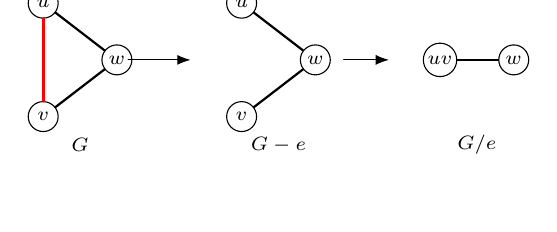
\begin{tikzpicture}[scale=0.72]
  \node[gv] (a1) at (0,1) {$u$}; \node[gv] (b1) at (0,-1) {$v$}; \node[gv] (c1) at (1.3,0) {$w$};
  \draw[thick] (a1)--(b1) (a1)--(c1) (b1)--(c1); \draw[very thick,red] (a1)--(b1);
  \node[draw=none,font=\scriptsize] at (0.65,-1.5) {$G$};
  \node[gv] (a2) at (3.5,1) {$u$}; \node[gv] (b2) at (3.5,-1) {$v$}; \node[gv] (c2) at (4.8,0) {$w$};
  \draw[thick] (a2)--(c2) (b2)--(c2); \node[draw=none,font=\scriptsize] at (4.15,-1.5) {$G-e$};
  \node[gv] (uv) at (7,0) {$uv$}; \node[gv] (c3) at (8.3,0) {$w$}; \draw[thick] (uv)--(c3);
  \node[draw=none,font=\scriptsize] at (7.65,-1.5) {$G/e$};
  \draw[->,>=Latex] (1.5,0)--(2.6,0); \draw[->,>=Latex] (5.3,0)--(6.1,0);
\end{tikzpicture}
\end{center}

\begin{theorem}[删除—收缩递推]\label{thm:delcont}
对图 $G$ 中任意边 $e$，$\;\chrom{G}{k}=\chrom{G-e}{k}-\chrom{G/e}{k}.$
\end{theorem}

\begin{proof}
考察 $G-e$ 的所有正常 $k$-着色，分两类：端点 $u,v$ \emph{异色}者恰为 $G$ 的正常着色，共 $\chrom{G}{k}$ 种；
端点 $u,v$ \emph{同色}者合并即得 $G/e$ 的正常着色，共 $\chrom{G/e}{k}$ 种。两类之和为 $\chrom{G-e}{k}$，
移项即得。\qed
\end{proof}

\begin{remark}
$G-e$ 和 $G/e$ 的边数都比 $G$ 少，所以递推迟早会落到没有边的图 $E_n$（$n$ 个孤立点），此时 $\chrom{E_n}{k}=k^{n}$。
把递推式一路反推回去，便知 $\chrom{G}{k}$ 确实是个多项式，命题~\ref{prop:basic}(1) 也由此得证。
\end{remark}

\begin{algorithm}[H]
\DontPrintSemicolon\SetKwFunction{FChrom}{Chromatic}
\KwIn{图 $G=(V,E)$，颜色数 $k$}\KwOut{$\chrom{G}{k}$}
\If{$E=\varnothing$}{\Return $k^{|V|}$\;}
任取 $e\in E$\;\Return $\FChrom(G-e,k)-\FChrom(G/e,k)$\;
\caption{用删除—收缩递推计算色多项式}
\end{algorithm}

\begin{remark}
这个算法每递推一次，子问题的数目就翻倍，最坏情况下要算 $O(2^{m})$ 个子图，因此一般图的色多项式
没有多项式时间算法（精确计数是 \#P-难的）。实际使用时，删除—收缩主要用于小图的手算，
或者结合一点粘贴、对称性等结构来减少递推次数。
\end{remark}

% =====================================================================
\section{常见图的色多项式}\label{sec:common}
% =====================================================================

\textbf{空图 $E_n$.}\, 顶点之间没有约束，$\chrom{E_n}{k}=k^{n}$。
\textbf{完全图 $K_n$.}\, 按任意顺序逐点染色，第 $i$ 个点要避开前面 $i-1$ 个点用过的颜色，所以
$\chrom{K_n}{k}=k(k-1)(k-2)\cdots(k-n+1)$。

\begin{theorem}\label{thm:tree}
若 $T$ 是 $n$ 阶树，则 $\chrom{T}{k}=k(k-1)^{n-1}$。
\end{theorem}
\begin{proof}
对 $n$ 归纳。$n=1$ 显然。$n>1$ 时取悬挂叶 $v$（邻点 $u$），$T-v$ 仍是 $n-1$ 阶树，其着色有
$k(k-1)^{n-2}$ 种；每种下叶 $v$ 仅须避开 $u$ 一色，有 $k-1$ 种。故 $\chrom{T}{k}=k(k-1)^{n-1}$。\qed
\end{proof}

特别地，路径 $P_n$ 也是树，$\chrom{P_n}{k}=k(k-1)^{n-1}$。
反过来也对：一个 $n$ 阶连通图的色多项式是 $k(k-1)^{n-1}$，当且仅当它是一棵树。
也就是说，单凭色多项式就能把树从所有连通图里区分出来。

\begin{theorem}\label{thm:cycle}
对 $n\ge 3$，$\chrom{C_n}{k}=(k-1)^{n}+(-1)^{n}(k-1)$。
\end{theorem}
\begin{proof}
取环上一边 $e$。$C_n-e$ 即路径 $P_n$，$\chrom{C_n-e}{k}=k(k-1)^{n-1}$；收缩 $e$ 得 $C_{n-1}$。
由定理~\ref{thm:delcont}，$\chrom{C_n}{k}=k(k-1)^{n-1}-\chrom{C_{n-1}}{k}$，初值
$\chrom{C_3}{k}=k(k-1)(k-2)$。设 $a_n=\chrom{C_n}{k}$，解一阶递推 $a_n=k(k-1)^{n-1}-a_{n-1}$
（乘 $(-1)^{n}$ 累加）得 $a_n=(k-1)^{n}+(-1)^{n}(k-1)$。\qed
\end{proof}

\subsection{轮图 $W_n$：闭式的应用}
轮图 $W_n$ 由一个 $(n-1)$-圈外加一个与圈上所有顶点相邻的中心点构成。中心点须与圈上各点异色，
故固定其颜色后，圈上 $n-1$ 个顶点只能用余下 $k-1$ 色作正常染色，即 $\chrom{C_{n-1}}{k-1}$。由定理~\ref{thm:cycle}，
\[
  \chrom{W_n}{k}=k\,\chrom{C_{n-1}}{k-1}
  =k\big[(k-2)^{n-1}+(-1)^{n-1}(k-2)\big].
\]
有了圈的闭式，轮图的色多项式可以直接写出来，不必再从边一条条递推。

\subsection{拼接图：不交并与一点粘贴}
两个图 $G,H$ 的不交并 $G\cup H$，着色互不影响，所以 $\chrom{G\cup H}{k}=\chrom{G}{k}\chrom{H}{k}$
（也就是命题~\ref{prop:basic}(3)）。如果 $G,H$ 只共用一个顶点 $v$、没有公共边（记作一点粘贴 $G\vee_{v}H$），
那么两边的着色必须在 $v$ 上取同一种颜色：固定 $v$ 的颜色之后，$G,H$ 各自还剩 $\chrom{G}{k}/k$、$\chrom{H}{k}/k$ 种染法，于是
\[
  \chrom{G\vee_{v}H}{k}=\frac{\chrom{G}{k}\,\chrom{H}{k}}{k}.
\]
拿这个公式去看“蝴蝶图”（两个三角形在一点粘成），它的色多项式直接就是
$[k(k-1)(k-2)]^{2}/k=k(k-1)^{2}(k-2)^{2}$。

\begin{center}
\begin{tikzpicture}[scale=0.62]
  \node[gv] (c) at (0,0){$v$};
  \node[gv] (a1) at (-1.2,0.95){}; \node[gv] (a2) at (-1.2,-0.95){};
  \node[gv] (b1) at (1.2,0.95){};  \node[gv] (b2) at (1.2,-0.95){};
  \draw[thick] (c)--(a1)--(a2)--(c) (c)--(b1)--(b2)--(c);
  \node[draw=none,font=\scriptsize] at (0,-1.7){蝴蝶图 $=$ 两 $K_3$ 一点粘贴};
\end{tikzpicture}
\end{center}

% =====================================================================
\section{计算实例：三角形带悬挂边}\label{sec:example}
% =====================================================================

以图 $G$（顶点 $\{1,2,3,4\}$，$12,23,31$ 构成 $K_3$，外加悬挂边 $34$）完整演示递推。

\begin{center}
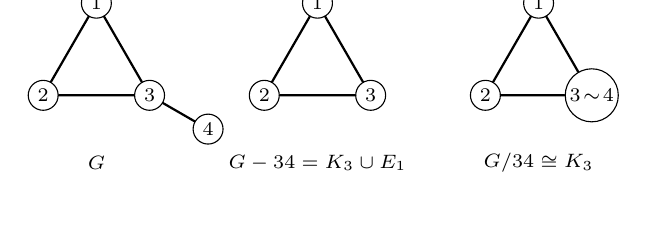
\begin{tikzpicture}[scale=0.78]
  \node[gv] (v1) at (90:1){$1$};\node[gv] (v2) at (210:1){$2$};
  \node[gv] (v3) at (330:1){$3$};\node[gv] (v4) at (330:2.1){$4$};
  \draw[thick] (v1)--(v2)--(v3)--(v1) (v3)--(v4);
  \node[draw=none,font=\scriptsize] at (0,-1.6){$G$};
  \begin{scope}[xshift=3.6cm]
    \node[gv] (a1) at (90:1){$1$};\node[gv] (a2) at (210:1){$2$};\node[gv] (a3) at (330:1){$3$};
    \draw[thick] (a1)--(a2)--(a3)--(a1);
    \node[draw=none,font=\scriptsize] at (0,-1.6){$G-34=K_3\cup E_1$};
  \end{scope}
  \begin{scope}[xshift=7.2cm]
    \node[gv] (b1) at (90:1){$1$};\node[gv] (b2) at (210:1){$2$};\node[gv] (b3) at (330:1){$3\!\sim\!4$};
    \draw[thick] (b1)--(b2)--(b3)--(b1);
    \node[draw=none,font=\scriptsize] at (0,-1.6){$G/34\cong K_3$};
  \end{scope}
\end{tikzpicture}
\end{center}

取悬挂边 $e=34$。删边后图退化为 $K_3$ 与孤立点 $4$ 的不交并，由命题~\ref{prop:basic}(3)
\[
  \chrom{G-34}{k}=\chrom{K_3}{k}\cdot\chrom{E_1}{k}=k(k-1)(k-2)\cdot k=k^{2}(k-1)(k-2);
\]
收缩 $34$ 恰得 $K_3$，$\chrom{G/34}{k}=k(k-1)(k-2)$。故
$\chrom{G}{k}=k^{2}(k-1)(k-2)-k(k-1)(k-2)=k(k-1)^{2}(k-2)$。
\textbf{验证：}先染 $K_3$ 共 $k(k-1)(k-2)$ 种，点 $4$ 避开邻点 $3$ 一色有 $k-1$ 种，
乘积恰为 $k(k-1)^{2}(k-2)$，与递推一致。\qed

\textbf{例 2.\,$K_4$ 减去一条边.}\, 设 $G=K_4-e$（即 $K_4$ 删去边 $34$），其边为
$12,13,14,23,24$，恰是两个三角形 $123$、$124$ 在边 $12$ 上的粘合（钻石图）。取现存边 $12$：
删去后 $(K_4-e)-12$ 仅余 $1\!-\!3\!-\!2\!-\!4\!-\!1$，即 $4$-圈 $C_4$；收缩 $12$ 使两端合一，
新点仍连 $3,4$，而 $34$ 不存在，故得 $3$ 阶路 $P_3$。于是递推\emph{一步}即落到已知图类：
\[
  \chrom{K_4-e}{k}=\chrom{C_4}{k}-\chrom{P_3}{k}
  =k(k-1)(k^{2}-3k+3)-k(k-1)^{2}=k(k-1)(k-2)^{2}.
\]
从结果里也能读出色数：$k=0,1,2$ 都是根，而 $k=3$ 时多项式为正，所以 $\chrnum(K_4-e)=3$
（理由见下节命题~\ref{prop:introot}）。这个例子和例 1 说明的是同一件事：只要挑准要递推的那条边，
往往一两步就能把图化归到已知图类上。

\begin{center}
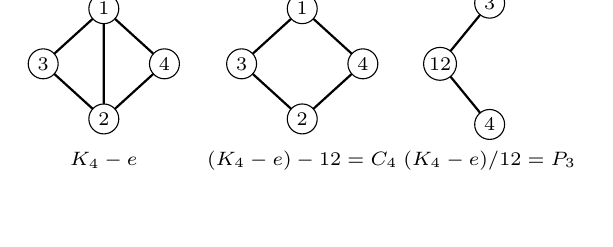
\begin{tikzpicture}[scale=0.7]
  \node[gv] (a) at (90:1){$1$};\node[gv] (b) at (270:1){$2$};
  \node[gv] (c) at (180:1.1){$3$};\node[gv] (d) at (0:1.1){$4$};
  \draw[thick] (a)--(b) (a)--(c) (b)--(c) (a)--(d) (b)--(d);
  \node[draw=none,font=\scriptsize] at (0,-1.75){$K_4-e$};
  \begin{scope}[xshift=3.6cm]
    \node[gv] (a2) at (90:1){$1$};\node[gv] (b2) at (270:1){$2$};
    \node[gv] (c2) at (180:1.1){$3$};\node[gv] (d2) at (0:1.1){$4$};
    \draw[thick] (a2)--(c2) (b2)--(c2) (a2)--(d2) (b2)--(d2);
    \node[draw=none,font=\scriptsize] at (0,-1.75){$(K_4-e)-12=C_4$};
  \end{scope}
  \begin{scope}[xshift=7.0cm]
    \node[gv] (m) at (180:0.9){$12$};\node[gv] (c3) at (90:1.1){$3$};\node[gv] (d3) at (270:1.1){$4$};
    \draw[thick] (m)--(c3) (m)--(d3);
    \node[draw=none,font=\scriptsize] at (0,-1.75){$(K_4-e)/12=P_3$};
  \end{scope}
\end{tikzpicture}
\end{center}

% =====================================================================
\section{色多项式与图结构}\label{sec:structure}
% =====================================================================

除了用来计数，色多项式的系数本身就带着不少图的信息。Whitney 给出的断集公式是
$\chrom{G}{k}=\sum_{F\subseteq E}(-1)^{|F|}k^{c(F)}$，其中 $c(F)$ 是子图 $(V,F)$ 的连通分支数。

\begin{theorem}[系数的符号与界]\label{thm:coeff}
设 $G$ 为 $n$ 阶简单图，则
$\chrom{G}{k}=k^{n}-m\,k^{n-1}+a_{2}k^{n-2}-a_{3}k^{n-3}+\cdots+(-1)^{n-1}a_{n-1}k$，
其中 $m=|E|$，诸 $a_i\ge 0$，即系数正负相间、常数项为 $0$。
\end{theorem}

\begin{proof}[证明梗概]
按 $|F|$ 分组求和：$|F|=0$ 给出 $k^{n}$；$|F|=1$（每条边使分支数减 $1$）给出 $-m\,k^{n-1}$；
一般项符号为 $(-1)^{|F|}$，分支数 $c(F)\ge 1$ 保证最低次为 $k^{1}$。\qed
\end{proof}

\begin{corollary}\label{cor:read}
由 $\chrom{G}{k}$ 可确定：顶点数 $n$（多项式次数）、边数 $m$（$k^{n-1}$ 系数的相反数）、
连通分支数 $c$（$k$ 的最高整除幂次 $k^{c}\,\|\,\chrom{G}{k}$）、色数 $\chrnum(G)$（最小非零项次数）。
\end{corollary}

\begin{proposition}[整数根]\label{prop:introot}
若 $G$ 含完全子图 $K_r$（即团数 $\omega(G)\ge r$），则 $0,1,\dots,r-1$ 都是 $\chrom{G}{k}$ 的根；
从而 $\chrnum(G)$ 恰为 $\chrom{G}{k}$ 的最小正整数根。
\end{proposition}
\begin{proof}
$K_r\subseteq G$ 蕴含 $\chrnum(G)\ge r$，故当 $k<r$ 时不存在正常 $k$-着色，$\chrom{G}{k}=0$，
即 $k=0,1,\dots,r-1$ 均为根。又 $\chrom{G}{\chrnum(G)}>0$，结合命题~\ref{prop:basic}(4) 得后半句。\qed
\end{proof}

\begin{remark}[色多项式不能完全确定图]
会有这样的情形：两个非同构图 $G,H$，色多项式却相同（$\chrom{G}{k}=\chrom{H}{k}$），称为色等价。
最简单的反例就出在树上——所有 $n$ 阶树的色多项式都是 $k(k-1)^{n-1}$，可它们未必同构。比如 5 阶的
路 $P_5$ 和星 $K_{1,4}$，最大度分别是 $2$ 和 $4$，结构差得很远，色多项式却都是 $k(k-1)^{4}$。
反过来问，什么样的图能被它的色多项式唯一确定（所谓色唯一图），至今还没有完整的回答。

\begin{center}
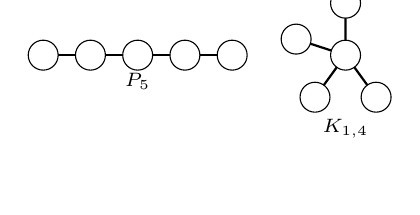
\begin{tikzpicture}[scale=0.6]
  \node[gv] (p1) at (0,0){}; \node[gv] (p2) at (1,0){};
  \node[gv] (p3) at (2,0){}; \node[gv] (p4) at (3,0){}; \node[gv] (p5) at (4,0){};
  \draw[thick] (p1)--(p2)--(p3)--(p4)--(p5);
  \node[draw=none,font=\scriptsize] at (2,-0.55){$P_5$};
  \begin{scope}[xshift=6.4cm]
    \node[gv] (c) at (0,0){}; \node[gv] (s1) at (90:1.1){};
    \node[gv] (s2) at (162:1.1){}; \node[gv] (s3) at (234:1.1){}; \node[gv] (s4) at (306:1.1){};
    \draw[thick] (c)--(s1) (c)--(s2) (c)--(s3) (c)--(s4);
    \node[draw=none,font=\scriptsize] at (0,-1.55){$K_{1,4}$};
  \end{scope}
\end{tikzpicture}
\end{center}
\end{remark}

\begin{remark}[与四色定理的联系]
按命题~\ref{prop:basic}(4)，四色定理等价于说：对任意平面图 $G$，都有 $\chrom{G}{4}>0$。
这其实就是 Birkhoff 当年引入色多项式时想做的事情——他想用多项式的语言去重新表述四色问题。
\end{remark}

% =====================================================================
\section{总结与展望}
% =====================================================================

本文从一个计数问题出发，定义了图的色多项式，并以删除—收缩递推 $\chrom{G}{k}=\chrom{G-e}{k}-\chrom{G/e}{k}$
作为主要工具，算出了完全图、树、环图、轮图等几类图的闭式。色多项式的系数也带着图的信息：
次数给出顶点数，$k^{n-1}$ 的系数给出边数，能整除的最高 $k$ 的幂给出连通分支数，最小的正整数根给出色数。
不过它也有局限：一方面，存在色等价的非同构图，色多项式并不能把图完全区分开；另一方面，
它的精确计算是 \#P-难的，所以它更像一个结构性的不变量，而不是一个高效的计数工具。

最后提一句，删除—收缩这种递推并不是色多项式独有的。Tutte 多项式
$T_G(x,y)=T_{G-e}(x,y)+T_{G/e}(x,y)$（$e$ 非环、非桥）用的是同一个递推，但在不同的取值下
统一了一批图计数问题：$T_G(1,1)$ 是生成树的数目，而 $\chrom{G}{k}=(-1)^{n-c}\,k^{c}\,T_G(1-k,0)$ 正是色多项式。
换句话说，色多项式其实是 Tutte 多项式的一个特例，本文讨论的递推不过是更一般理论里的一个片段。

\end{document}
